\chapter{Analyse du projet}
La résolution comporte deux parties :\begin{itemize}
\item le calcul des couples d'indices qui seront reliés\ ;
\item le calcul du chemin reliant chaque couple d'indices.
\end{itemize}

\section{Calcul des couples d'indices }

Cette partie de la résolution comporte trois sous-problèmes:
\begin{itemize}
\item le calcul des ensembles de voisins\ ;
\item la propagation des ensembles de voisins\ ;
\item le est d'existence de chemin.
\end{itemize}

\subsection{Calcul des ensembles de voisins}

Pour chaque indice, on calcule l'ensemble des indices auxquels il peut être relié (appelé par la suite ensemble des voisins possibles).
Deux indices sont des voisins possibles si :
\begin{itemize}
\item ils ont la même valeur d'indice\ ;
\item leur distance ($abs(x_1-x_2)+abs(y_1-y_2)+1$ pour deux indices de coordonnées $(x_1,y_1)$ et $(x_2,y_2)$) est inférieure et a la même parité que leur valeur d'indice.
\end{itemize}

Ces conditions sont des conditions nécessaires à l'existence d'un chemin liant les deux indices, mais pas suffisantes.
Les couples impossibles seront progressivement éliminés par les analyses suivantes jusqu'à ce que chaque indice n'ait plus qu'un voisin.

\begin{figure}[h]
\centering
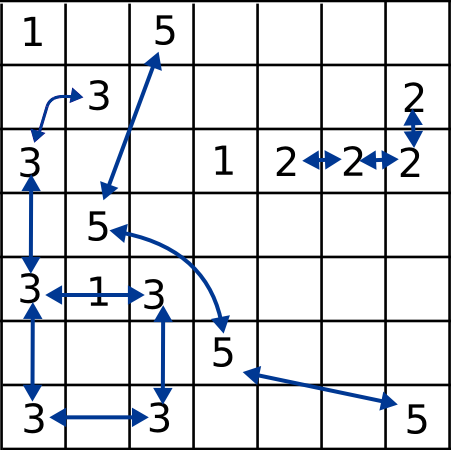
\includegraphics[scale=0.25]{voisins}
\caption{Ensembles de voisins.}
\end{figure}

\subsection{Formation des couples}

Au cours de la résolution du problème le solveur devra parvenir à retrouver les couples, c'est-à-dire associer chaque indice à son unique voisin.

Lorsqu'un indice $c_1$ n'a qu'un voisin $c_2$, $c_1$ et $c_2$ forment un couple.

$c_2$ ne peut plus former de couple avec un autre indice, il faut donc supprimer $c_2$ des autres ensembles de voisins possibles.

Cette suppression peut entraîner la formation de nouveaux couples. En effet, il est possible que parmi les indices qui n'ont plus $c_2$ pour voisin, certains ne comportent plus qu'un seul autre voisin (figure \ref{affectation1}). 

\begin{figure}[h]

  \centering  
  \subfloat[$c_1$ a $c_2$ pour unique voisin. ]{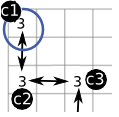
\includegraphics[scale=1]{affectation1}}
  \subfloat[$c_1$ et $c_2$ forment donc un couple. À son tour $c_3$ n'a plus qu'un voisin, avec lequel il forme donc un couple.]{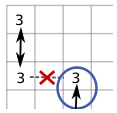
\includegraphics{affectation2}}
  \caption{Affectation des couples}
  \label{affectation1}
\end{figure}

Pour certains problèmes cette phase de propagation suffit à déterminer l'ensemble des couples.

Dans le cas général il faut raffiner les ensembles de voisins en vérifiant l'existence de chemins.

\subsection{Test de l'existence d'un chemin entre deux cases}

Au cours de la résolution, il sera nécessaire de tester l'existence d'un chemin entre deux coordonnées. Cela permettra notamment d'éliminer des couples potentiels.

Lorsqu'un indice $c_1$ possède plusieurs voisins, on vérifie pour chacun d'entre eux s'il existe au moins un chemin le liant à $c_1$ dans la grille. 

Un chemin est constitué d'une suite de cases : la première case est la case de départ, et les cases suivantes conduisent à la case d'arrivée. 

Ce chemin ne doit passer que par des cases libres. Une case est libre si elle ne correspond pas à une case indice et si elle n'est empruntée par aucun chemin.

La longueur du chemin doit être égale à la valeur des indices.

Pour tester l'existence d'un chemin, on peut ainsi partir de la case de départ puis ajouter une case suivante, selon les conditions suivantes : 
\begin{itemize}
\item la case doit être une case adjacente de la case précédente\ ;
\item la case ne doit pas  être déjà occupée par un autre chemin ou un autre indice\ ;
\item la case ne doit pas déjà faire partie du chemin\ ; en effet le chemin ne doit pas se recouper.
\end{itemize}
On continue ainsi récursivement jusqu'à arriver à la case d'arrivée ou bien à un chemin trop long.

Ce test permet de réduire les ensembles de voisins et ainsi, avec la phase de propagation, de découvrir de nouveaux couples d'indices.

\section{Calcul du chemin entre un couple d'indices}

Il est utile de déterminer par quelles cases passe le chemin qui relie un couple.

En effet, aucun autre chemin ne pourra emprunter ces cases. Cela pourra donc permettre l'élimination de certains couples de voisins lors de la suite de l'exécution du programme (figure \ref{calcul-chemin}).
\begin{figure}[h]
  \centering  
  \subfloat[Les deux indices 4 sont un couple de voisins possibles.]{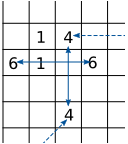
\includegraphics[scale=0.5]{constr-elim-1}}
 \hspace {1cm}
  \subfloat[Après la construction du début de chemin entre les deux 6, il n'y a plus de chemin valide entre les deux quatres.]{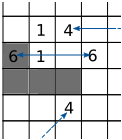
\includegraphics[scale=0.5]{constr-elim-2}}
  \caption{Le calcul de chemin permet d'éliminer des voisins possibles.}
  \label{calcul-chemin}
\end{figure}


Lorsque plusieurs chemins relient un couple d'indices ($c_1$, $c_2$), on ne peut pas choisir a priori l'un d'entre eux. Cependant dans le cas où tous ces chemins ont un préfixe commun, on peut marquer les cases de cet unique début de chemin comme étant occupées (figure \ref{progression-chemin}).

\begin{figure}[h]
  \centering  
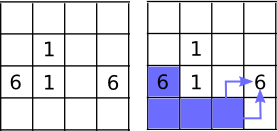
\includegraphics[scale=0.5]{construire}
\caption{Dans cet exemple, seules les quatre premières cases du chemin peuvent être construites. Au delà, il y a plus d'une possibilité.}
\label{progression-chemin}
\end{figure}

S'il y a un unique début de chemin, il passe forcément par une des quatre cases adjacentes de $c_1$. Pour chaque case adjacente on peut alors tester l'existence d'un chemin la reliant à l'indice d'arrivée. S'il y a plus d'une case possible, il n'y a pas de début unique de chemin. Sinon on a trouvé un unique début de chemin. On peut ensuite recommencer le même test à partir de cette case de manière récursive. 


Si $c_3$ est l'extrémité du préfixe de tous les chemins entre $c_1$ et $c_2$, il reste à découvrir le chemin de $c_3$ à $c_2$. Pour mémoriser cette information, on remplace l'indice $c_1$ par le nouvel indice $c_3$ et on remplace le couple d'indices
($c_1$, $c_2$) par le couple $(c_3, c_2)$ (figure \ref{remplacement-couple}).

\begin{figure}[h]
  \centering  
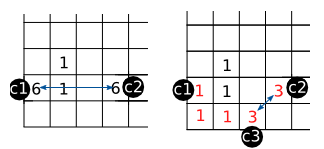
\includegraphics[scale=0.5]{remplacement}
\caption{le couple
d’indices $(c_1, c_2)$ est remplacé par le couple $(c_3, c_2)$.}
\label{remplacement-couple}
\end{figure}

\section{Enchaînement des traitements}

Les deux parties (calcul des couples d'indices, calcul des chemins) sont
interdépendantes : lorsqu'un nouveau couple d'indices est trouvé, il
faut rechercher le chemin les reliant et la découverte d'un nouveau
chemin ou d'une partie de chemin permet de trouver de nouveaux couples
d'indices.

L'enchaînement de ces deux traitements se fait selon l'algorithme suivant :
\begin{algorithm}
Calculer les ensembles de voisins initiaux (calculés avec la distance) \;
Propager les ensembles de voisins \;
\Repeter{pas de modification de la grille}{Reduire les ensembles de voisins en vérifiant l'existence de chemins \;
Propager les ensembles de voisins \;
\ForEach{couple d'indices non reliés par un chemin}{Rechercher un chemin entre les deux indices \;
Mettre à jour la grille des cases occupées \;}
}
\caption{Enchainement des traitements}
\end{algorithm}
